\PassOptionsToPackage{table}{xcolor}
\documentclass{article}
\usepackage[colorlinks]{hyperref}
\usepackage[margin=1.25in]{geometry}
\usepackage{amsmath,amssymb,amsthm,booktabs,tikz}
\usepackage[final]{microtype}
\usepackage{libertine}
\usepackage[varqu]{zi4}
\usepackage[libertine]{newtxmath}
\usepackage[T1]{fontenc}
\usepackage[utf8]{inputenc}
\usepackage{tabto}
\usepackage[normalem]{ulem}

\usetikzlibrary{shapes.multipart}

% Seven colors safe for use color blindness.
% Colors taken from doi:10.1038/nmeth.1618.
\definecolor{cbOrange}{RGB}{230,159,0}
\definecolor{cbSkyBlue}{RGB}{86,180,233}
\definecolor{cbBluishGreen}{RGB}{0,158,115}
\definecolor{cbBlue}{RGB}{0,114,178}
\definecolor{cbVermillion}{RGB}{213,94,0}
\definecolor{cbReddischPurple}{RGB}{204,121,167}
\definecolor{cbYellow}{RGB}{240,228,66}

\theoremstyle{definition}
\newtheorem{problem}{Problem}
\newenvironment{questions}{\begin{enumerate}
\renewcommand{\theenumi}{P\arabic{problem}.\arabic{enumi}}}{\end{enumerate}}
\newcommand{\HL}[1]{\textcolor{cbReddischPurple}{#1}}

\newcommand{\abs}[1]{\lvert #1 \rvert}
\newcommand{\OOG}[1]{\mathord{\sim}#1}
\DeclareMathOperator{\bdiv}{div}

\newcommand{\BigO}[1]{\mathcal{O}\left(#1\right)}
\newcommand{\BigOmega}[1]{\Omega\left(#1\right)}
\newcommand{\BigTheta}[1]{\Theta\left(#1\right)}


\newcommand{\True}{\texttt{true}}
\newcommand{\False}{\texttt{false}}

%% Tikz
\usepackage{tikz}
\usetikzlibrary{arrows.meta,calc,decorations.pathreplacing,shapes.geometric,shapes.multipart,overlay-beamer-styles}
\tikzset{
    >=Stealth,
    dot/.style={circle,scale=0.35,draw=black,fill=black},
    stacked/.style={above,rectangle split,draw,rectangle split parts=#1,font=\strut,rectangle split part fill={none,black!10}},
    centered/.append style={align=center}
}


% Algorithm
\usepackage{algorithmic}
\newcommand{\GETS}{:=}
\newcommand{\VAR}[1]{\textit{#1\/}}
\newcommand{\AName}[1]{\textsc{#1}}
\renewcommand{\algorithmicrequire}{\textbf{Input:}}
\renewcommand{\algorithmicensure}{\textbf{Result:}}
\newcommand{\CMT}[1]{\text{``#1''}}
\renewcommand{\algorithmiccomment}[1]{\CMT{#1}}
\newcommand{\INV}[1]{\emph{inv: } #1}
\newcommand{\VF}[1]{\emph{bf: } #1}
\makeatletter
\newlength{\Algo@MyTabLength}
\newcommand{\AlgoTabTo}[1]{%
    \setlength{\Algo@MyTabLength}{#1}%
    \addtolength{\Algo@MyTabLength}{-\ALC@tlm}%
    \tabto{\Algo@MyTabLength}%
}
\newenvironment{myonlyalgo}[1][0]{
    \vskip 5pt
    \hrule
    \smallskip
    \begin{algorithmic}[1]
    \setcounter{ALC@line}{#1}
}{
    \end{algorithmic}
    \hrule
    \vskip 5pt
}
\newenvironment{myalgo}[2][0]{
    \vskip 5pt
    \hrule
    \smallskip
    \noindent{\textbf{Algorithm} #2\textbf{:}}
    \begin{algorithmic}[1]
    \setcounter{ALC@line}{#1}
}{
    \end{algorithmic}
    \hrule
    \vskip 5pt
}







%% Metadata
\newcommand{\Assignment}[1]{
    \title{\vskip-2em%The standard article.cls package puts 2em whitespace on top of the title, undo this.
           Assignment #1\\{\Large SFWRENG 2CO3: Data Structures and Algorithms--Winter 2023}}}
\newcommand{\Deadline}[1]{
    \author{Deadline: #1}
}
\date{{\normalsize
    Department of Computing and Software\\
    McMaster University
}}

\newcommand{\Warning}[1]{\textbf{\textcolor{red!80!black}{#1}}}
\renewcommand{\labelitemi}{$\blacktriangleright$}

\newcommand{\DEFAULTMSG}{
Please read the \emph{Course Outline} for the general policies related to assignments.
\begin{center}
\Warning{Plagiarism is a \underline{\textit{\vphantom{y}serious academic offense}} and will be handled accordingly.}\\
\Warning{All suspicions will be reported to the \underline{\textit{Office of Academic Integrity}}\\(in accordance with the \href{https://secretariat.mcmaster.ca/app/uploads/Academic-Integrity-Policy-1-1.pdf}{Academic Integrity Policy}).}
\end{center}

This assignment is an \emph{individual} assignment: do not submit work of others. All parts of your submission \emph{must} be your own work and be based on your own ideas and conclusions. Only \emph{discuss or share} any parts of your submissions with your TA or instructor.  You are \emph{responsible for protecting} your work: you are strongly advised to password-protect and lock your electronic devices (e.g., laptop) and to not share your logins with partners or friends! If you \emph{submit} work, then you are certifying that you have completed the work for this assignment by yourself. By submitting work, you agree to automated and manual plagiarism checking of all submitted work.

\emph{Late submission policy}. Late submissions will receive a late penalty of 20\% on the score per day late (with a five hour grace period on the first day, e.g., to deal with technical issues) and submissions five days (or more) past the due date are not accepted. In case of technical issues while submitting, contact the instructor \emph{before} the deadline.}

\newcommand{\SUBMITMSG}{\section*{Assignment Details}
Write a report in which you solve each of the above problems. Your submission:
\begin{enumerate}
\item must be a \texttt{PDF} file;
\item must have clearly labeled solutions to each of the stated problems;
\item must be clearly presented;
\item must \emph{not} be hand-written: prepare your report in \LaTeX{} or in a word processor such as Microsoft Word (that can print or exported to \texttt{PDF}).
\end{enumerate}
\Warning{Submissions that do not follow the above requirements will get a grade of zero.}}

\newcommand{\DEFAULTGRADING}{\section*{Grading}
Each problem counts equally toward the final grade of this assignment.
}

\usepackage{amsmath}

\Assignment{3}
\Deadline{March 5, 2023}
\begin{document}
\maketitle
\DEFAULTMSG{}

\begin{problem}
Consider the sequence of values $S = [12, 44, 13, 88, 23, 94, 11, 39, 20, 16, 5]$.
\begin{questions}

\item Draw the binary search tree obtained by adding the values in $S$ in sequence.

\begin{tikzpicture}
  \node[dot] (p) at (0, 0)       {};
  \node[dot] (l) at (-2, -1)     {}  edge[<-] (p);
  \node[dot] (ll) at (-3, -2)  {}  edge[<-] (l);
  \node[dot] (r) at (2, -1)     {}  edge[<-] (p);
  \node[dot] (rl) at (1, -2)  {}  edge[<-] (r);
  \node[dot] (rr) at (3, -2) {} edge[<-] (r);
  \node[dot] (rrr) at (3.5, -3) {} edge[<-] (rr);
  \node[dot] (rlr) at (1.5, -3) {} edge[<-] (rl);
  \node[dot] (rlrr) at (2, -4) {} edge[<-] (rlr);
  \node[dot] (rlrl) at (1, -4) {} edge[<-] (rlr);
  \node[dot] (rlrll) at (0.5, -5) {} edge[<-] (rlrl);

  \node[above left] at (p)  {12};
  \node[above left] at (l)  {11};
  \node[above left] at (ll) {5};
  \node[above right] at (r)  {44};
  \node[above left] at (rl) {13};
  \node[above right] at (rr) {88};
  \node[above right] at (rrr) {94};
  \node[above right] at (rlr) {23};
  \node[above right] at (rlrr) {39};
  \node[above left] at (rlrl) {20};
  \node[above left] at (rlrll) {16};
\end{tikzpicture}

\item Draw the red-black tree obtained by adding the values in $S$ in sequence.

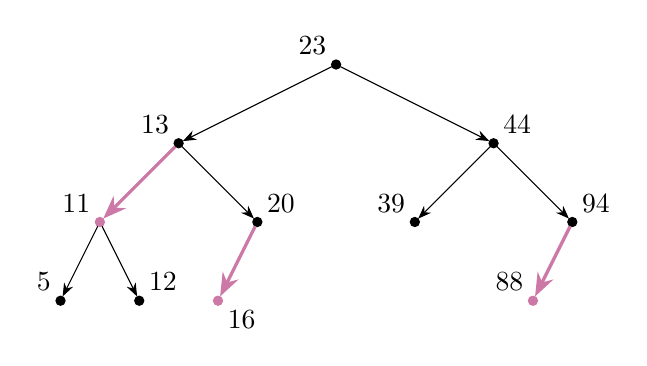
\begin{tikzpicture}
  \node[dot] (p) at (0, 0)       {};
  \node[dot] (l) at (-2, -1)     {}  edge[<-] (p);
  \node[dot,cbReddischPurple] (ll) at (-3, -2)  {}  edge[<-,very thick,cbReddischPurple] (l);
  \node[dot] (lll) at (-3.5, -3) {}  edge[<-] (ll);
  \node[dot] (llr) at (-2.5, -3) {}  edge[<-] (ll);
  \node[dot] (lr) at (-1, -2)  {}  edge[<-] (l);
  \node[dot,cbReddischPurple] (lrl) at (-1.5, -3)  {}  edge[<-,very thick,cbReddischPurple] (lr);
  \node[dot] (r) at (2, -1)     {}  edge[<-] (p);
  \node[dot] (rl) at (1, -2)  {}  edge[<-] (r);
  \node[dot] (rr) at (3, -2) {} edge[<-] (r);
  \node[dot,cbReddischPurple] (rrl) at (2.5, -3) {} edge[<-,very thick,cbReddischPurple] (rr);


  \node[above left] at (p)  {23};
  \node[above left] at (l)  {13};
  \node[above left] at (ll) {11};
  \node[above left] at (lll) {5};
  \node[above right] at (llr) {12};
  \node[below right] at (lrl) {16};
  \node[above right] at (lr) {20};
  \node[above right] at (r)  {44};
  \node[above left] at (rl) {39};
  \node[above right] at (rr) {94};
  \node[above left] at (rrl) {88};
\end{tikzpicture}

\item Consider the hash-function $h(k) = (2k + 5) \bmod 11$ and a hash-table of $11$ table entries that uses hashing with separate chaining. Draw the hash-table obtained by adding the values in $S$ in sequence.

\begin{tikzpicture}
  \node[hlisted=11,text width=1cm] (ar) {
  \Null{}
  \nodepart{two}\At{A128}
  \nodepart{three}\Null{}
  \nodepart{four}\Null{}
  \nodepart{five}\At{C923}
  \nodepart{six}\At{9D21}
  \nodepart{seven}\At{ADF3}
  \nodepart{eight}\At{F923}
  \nodepart{nine}\Null{}
  \nodepart{ten}\At{E00F}
  \nodepart{eleven}\Null{}};
  
  \node[above] at (ar.north) {$L[0\dots11)$:};
  \node[left] at (ar.one west) {0:};
  \node[left] at (ar.two west) {1:};
  \node[left] at (ar.three west) {2:};
  \node[left] at (ar.four west) {3:};
  \node[left] at (ar.five west) {4:};
  \node[left] at (ar.six west) {5:};
  \node[left] at (ar.seven west) {6:};
  \node[left] at (ar.eight west) {7:};
  \node[left] at (ar.nine west) {8:};
  \node[left] at (ar.ten west) {9:};
  \node[left] at (ar.eleven west) {10:};


  \node[lnode,right=0.4cm,yshift=0cm,scale=0.65] (n3) at (ar.one east) {item: {20}\nodepart{two}next: \Null};
  \node[above right,scale=0.65] at (n3.north west) {\At{A128}:};
  \path (ar.two east) edge[->] (n3.north west);




  \node[lnode,right=0.4cm,yshift=0cm,scale=0.65] (n1) at (ar.three east) {item: {5}\nodepart{two}next: \At{312C}};
  \node[above right,scale=0.65] at (n1.north west) {\At{C923}:};
  \path (ar.five east) edge[->] (n1.north west);

  \node[lnode,right=0.4cm,scale=0.65] (n2) at (n1.east) {item: {16}\nodepart{two}next: \Null};
  \node[above right,scale=0.65] at (n2.north west) {\At{312C}:};
  \draw[->] (n1.two east) -| ($(n1.text split)!0.5!(n2.text split)$) |- (n2.north west);




  \node[lnode,right=0.4cm,yshift=0cm,scale=0.65] (n4) at (ar.five east) {item: {11}\nodepart{two}next: \At{1D23}};
  \node[above right,scale=0.65] at (n4.north west) {\At{9D21}:};
  \path (ar.six east) edge[->] (n4.north west);

  \node[lnode,right=0.4cm,scale=0.65] (n5) at (n4.east) {item: {88}\nodepart{two}next: \At{5283}};
  \node[above right,scale=0.65] at (n5.north west) {\At{1D23}:};
  \draw[->] (n4.two east) -| ($(n4.text split)!0.5!(n5.text split)$) |- (n5.north west);

  \node[lnode,right=0.4cm,scale=0.65] (n6) at (n5.east) {item: {44}\nodepart{two}next: \Null};
  \node[above right,scale=0.65] at (n6.north west) {\At{5283}:};
  \draw[->] (n5.two east) -| ($(n5.text split)!0.5!(n6.text split)$) |- (n6.north west);



  \node[lnode,right=0.4cm,yshift=0cm,scale=0.65] (n7) at (ar.seven east) {item: {39}\nodepart{two}next: \At{DE92}};
  \node[above right,scale=0.65] at (n7.north west) {\At{ADF3}:};
  \path (ar.seven east) edge[->] (n7.north west);

  \node[lnode,right=0.4cm,scale=0.65] (n8) at (n7.east) {item: {94}\nodepart{two}next: \Null};
  \node[above right,scale=0.65] at (n8.north west) {\At{DE92}:};
  \draw[->] (n7.two east) -| ($(n7.text split)!0.5!(n8.text split)$) |- (n8.north west);
  



  \node[lnode,right=0.4cm,yshift=0cm,scale=0.65] (n9) at (ar.nine east) {item: {23}\nodepart{two}next: \At{6A43}};
  \node[above right,scale=0.65] at (n9.north west) {\At{F923}:};
  \path (ar.eight east) edge[->] (n9.north west);

  \node[lnode,right=0.4cm,scale=0.65] (n10) at (n9.east) {item: {12}\nodepart{two}next: \Null};
  \node[above right,scale=0.65] at (n10.north west) {\At{6A43}:};
  \draw[->] (n9.two east) -| ($(n9.text split)!0.5!(n10.text split)$) |- (n10.north west);



  \node[lnode,right=0.4cm,yshift=0cm,scale=0.65] (n11) at (ar.eleven east) {item: {13}\nodepart{two}next: \Null};
  \node[above right,scale=0.65] at (n11.north west) {\At{E00F}:};
  \path (ar.ten east) edge[->] (n11.north west);

\end{tikzpicture}

\item Consider the hash-function $h(k) = (3k + 2) \bmod 11$ and a hash-table of $11$ table entries that uses hashing with linear probing. Draw the hash-table obtained by adding the values in $S$ in sequence.

\begin{tikzpicture}
  \node[hlisted=11,text width=1cm] (ar) {
  16
  \nodepart{two}5
  \nodepart{three}44
  \nodepart{four}88
  \nodepart{five}11
  \nodepart{six}12
  \nodepart{seven}23
  \nodepart{eight}20
  \nodepart{nine}13
  \nodepart{ten}94
  \nodepart{eleven}39};
  
  \node[above] at (ar.north) {$L[0\dots11)$:};
  \node[left] at (ar.one west) {0:};
  \node[left] at (ar.two west) {1:};
  \node[left] at (ar.three west) {2:};
  \node[left] at (ar.four west) {3:};
  \node[left] at (ar.five west) {4:};
  \node[left] at (ar.six west) {5:};
  \node[left] at (ar.seven west) {6:};
  \node[left] at (ar.eight west) {7:};
  \node[left] at (ar.nine west) {8:};
  \node[left] at (ar.ten west) {9:};
  \node[left] at (ar.eleven west) {10:};

\end{tikzpicture}

\end{questions}
\end{problem}


\begin{problem}
We say that a hash function $h : \mathcal{U} \rightarrow \mathbb{N}$ that maps values from a set $\mathcal{U}$ to integers in the range $[0\dots M)$ is \emph{$n$-perfect} if there exists at most $n$ distinct values $u_1, \dots, u_j \in \mathcal{U}$ such that $h(u_1) = \dots = h(u_j)$.
\begin{questions}
\item Consider the hash function $h(k) = (2k + 5) \bmod 11$. Is this hash function $2$-perfect for the inputs $0, \dots, 21$? Explain why or why not.

\textbf{Answer:}
This function is 2-perfect for the inputs 0,...,21 since after computation, there is only 2 values mapped to one spot in the hash table. In summary, since the function has 2k, as you loop through the values, the new value will most often be 2 more than the previous. This is until you hit 11 as it is mod 11, then it will start back at either 0 or 1 depending on if the previous value was 9 or 10. The following is the computation.\\

\begin{center}
  \begin{tabular}{||c|c|c|c|c|c|c|c||} 
    \hline
    v & h(v)=(2v+5)mod 11 & v & h(v) & v & h(v) & v & h(v) \\ [0.5ex] 
    \hline\hline
    0 & 5 & 6 & 6 & 12 & 7 & 18 & 8\\ 
    1 & 7 & 7 & 8 & 13 & 9 & 19 & 10 \\
    2 & 9 & 8 & 10 & 14 & 0 & 20 & 1 \\
    3 & 0 & 9 & 1 & 15 & 2 & 21 & 3 \\
    4 & 2 & 10 & 3 & 16 & 4 &  & \\
    5 & 4 & 11 & 5 & 17 & 6 &  & \\ [1ex] 
    \hline
  \end{tabular}
\end{center}

Rearrange to see that there are only two values per mapping. We can see that if there was 1 more value, it would no longer be 2-perfect:

\begin{center}
  \begin{tabular}{||c|c|c|c|c|c|c|c||} 
    \hline
    h(v) & v & h(v) & v & h(v) & v & h(v) & v \\ [0.5ex] 
    \hline\hline
    0 & 3, 14 & 3 & 10, 21 & 6 & 6, 17 & 9 & 13, 2\\ 
    1 & 9, 20 & 4 & 5, 16 & 7 & 12, 1 & 10 & 8, 19 \\
    2 & 4, 15 & 5 & 11, 0 & 8 & 7, 18 &  &  \\ [1ex] 
    \hline
  \end{tabular}
\end{center}


\item Prove that a hash function $h : \mathcal{U} \rightarrow \mathbb{N}$ can only be $n$-perfect if $\abs{\mathcal{U}} \leq n \cdot M$.

\textbf{Answer:}

Assume $h : \mathcal{U} \rightarrow \mathbb{N}$ is n-perfect and let 
$u_1, \dots, u_j$ be j distinct values in $\mathcal{U}$ such that $h(u_1) = \dots = h(u_j)$. Then we will have that $j \leq n$.

$\mathcal{S}_i = \{x \in \mathcal{U}\:|\:h(x) = i\}$ --> In other words, $\mathcal{S}_i$ has elements in $\mathcal{U}$ that map to $i$

This means, $\mathcal{U} = \sum_{i=0}^{M-1} \mathcal{S}_i$ where $|\mathcal{U}| = M$

since $h$ is n-perfect, we know $|\mathcal{S}_i| \leq n$

$\mathcal{U} = \sum_{i=0}^{M-1} \mathcal{S}_i$\\
$|\mathcal{U}| = |\sum_{i=0}^{M-1} \mathcal{S}_i|$\\
$ = \sum_{i=0}^{M-1} |\mathcal{S}_i|$\\
$ \leq \sum_{i=0}^{M-1} n$\\
$ = nM $\\

In conclusion, we have proven that assuming $h : \mathcal{U} \rightarrow \mathbb{N}$ is a n-perfect hash function, then $|\mathcal{U}| \leq nM$ holds.

As we provided an upper bound on the number of elements in $\mathcal{U}$ that can be hashed without collisions, we know that adding any more elements will result in more than n values being mapped to a single hash value, which violates n-perfect rules.

\item Can a general purpose hash function be $n$-perfect for any $M$? Argue why or why not.

\textbf{Answer: }

No a general-purpose hash function cannot be n-perfect for any M because a general-purpose hash function must be able to take in any set of input and ensure each hash value contains $\leq n$ values from the input. 
This means it needs to handle inputs such as lists that have a near infinite number of values (huge, but finite M), which is nearly impossible to be n-perfect as you'd have to consider infinite different inputs.

Let's take the set of all strings for example as what our hash function is hashing. There is no function we can provide that will perfectly distribute every string possible as even if our hash table is semi-filled, and we go to hash string x. I can append "a" (or any new string that will hash it to a collision) to x and that will mess up the function, thus resulting in a collision, violating the n-perfect rule.


\end{questions}
\end{problem}

\begin{problem}
Consider non-empty binary search trees $T_1$ and $T_2$ such that all values in $T_1$ are smaller than the values in $T_2$. The \AName{SetUnion} operation takes binary search trees $T_1$ and $T_2$ and returns a binary search trees holding all values originally in $T_1$ and $T_2$ (destroying $T_1$ and $T_2$ in the process). 
\begin{questions}
\item Assume the binary search trees storing $T_1$ and $T_2$ have the same height $h$. Show how to implement the \AName{SetUnion} operation in $\OOG{h}$ such that the resulting tree has a height of at-most $h+1$.

1) Remove max value in $T_1$ and store it in variable m\\
$h$ is worst-case time complexity, where the max value is at the $h_{th}$ level in the tree. $T_1$ will still have a height of $h$ or $h-1$ if max value m was the only value in level $h$ of the tree.

2) Add the max value m as the root of $T_1$\\
$\sim 1$ time complexity, as it just takes a little pointer logic. Make m node root of $T_1$ and make m.left be the old root of $T_1$. This will lead the tree be max height $h+1$ as we are only added 1 level (the new root) to the tree.
Also, we know all values in $T_1$ are smaller than m, so BST properties remain as we add $T_1$ as the left subtree of the new root, m.
At this point, $T_1$ is of height $ \leq h+1$ and $T_2$ is of height $h$

3) Take the root of $T_2$ and make it right subtree of new $T_1$\\
Again $\sim 1$ time complexity, as it just requires to make m.right $ = T_2$. We know the left subtree of m is max $h$ height and the right subtree is $h$ since we just added $T_2$ which is a tree of height $h$.
We also know that all values in $T_2$ are greater than the values in the current $T_1$, including the root. This allows us to put the root of $T_2$ as the right child of m, ensuring we keep BST properties.

4) return $T_1$\\

To conclude, the resulting tree will be of height $h+1$ since we took 2 tree of height $h$ and added 1 level to it (the root). We also know it keeps BST properties as we know all values in $T_2$ are larger than the maximum value in $T_1$, which allows us to put $T_2$ in the right subtree of the root of new $T_1$

\item Assume that $T_1$ and $T_2$ are red-black trees with the same black height $h$. Show how to implement a \AName{SetUnion} operation that returns a red-black tree in $\OOG{h}$.

1) Check height $h$ of tree, for step 5 (can be any since both are height $h$)\\
Takes $\OOG{h}$ since you just traverse the tree downwards once.

2) Remove min value in $T_2$ and store it in variable $m$\\
Removing the min value is max a $2h$ complexity function which is $\OOG{h}$. This is because you might need to traverse the longest path in the tree and given the tree can be 1 red node then 1 black, this could be of height $2h$.
Also, removing 1 node from the tree $T_2$ can result in the new height, $h_{new}$ to be either $h$ or $h-1$.

3) Calculate black height of $T_2$ and store it as $h_{new}$\\
This is $\OOG{h_{new}}$ which is $\leq \OOG{h}$ as you must traverse the entire tree once. 

4) Make the min value of $T_2$, $m$, the root of our new tree $T_3$\\
This is $\OOG{1}$ operation.

5) Make $T_1$ the left subtree of the root of $T_3$, $m$ and $T_2$ the right subtree\\
This is $\OOG{1}$ operation again as it's pointer manipulation. 
This is also correct as we know all values in $T_1$ were smaller than m, and all remaining values in $T_2$ are larger than m.

6) Fix tree: if $h_{new} = h$ then make both edges from the root black. If $h_{new} = h-1$ then make the left edge from the root red.\\
This is a $\OOG{1}$ operation as it requires performing 1 check and changing a single edge/node color. 

\item Assume that $T_1$ and $T_2$ are red-black trees with black heights $h_1 > h_2$. Show how to implement a \AName{SetUnion} operation that returns a red-black tree in $\OOG{h_1}$.

1) Check $h_1$ and $h_2$ of the trees\\
Takes $\OOG{h_1}$ since you just traverse both trees downwards once and the larger tree is of height $h_1$.

2) Traverse the right subtree of $T_1$ by $\frac{h_2}{2}$ rounded up (remember this rounding up instead of down for step 4). Get the node at that point.\\
This takes $\OOG{h_2} \leq h_1$.
We do this since we want to add a subtree of height $h_2$ ($T_2$) to the right subtree of $T_1$.
In this way, since the left and right subtrees of $T_1$ currently have height of $h_1$, if we take $\frac{1}{2} h_2$ from the right subtree and move it to the left, the left will now be $h_1 + \frac{1}{2} h_2$.
The right subtree is now $h_1 - \frac{1}{2} h_2$. When we go to add $T_2$ to the right subtree, it will make it $h_1 - \frac{1}{2} h_2 + h_2 = h_1 + \frac{1}{2} h_2$, which is the same height as the left subtree.
We will call this new height $h_3$

3) As explained in step 2, make the node found in step 2 the root of $T_1$ by performing the correct local rotations to maintain the left-leaning property and BST property of the tree (Note: the black height will be messed up). Insert $T_2$ in the rightmost subtree of $T_1$.\\
Since we are making a node somewhere in the farthest right path that is $\frac{1}{2} h_2$ down the tree, all the paths to the left of that but still in the right subtree might not be of the proper black height $h_3$.
This is $\OOG{h_2} \leq h_1$ time to perform the rotations and $\OOG{1}$ time for the insertion of $T_2$. 

4) To fix the ruined black-height in step 3: delete and reinsert the nodes left over in between the left subtree and far-right path if they are not length $h_3$.\\
This is $\OOG{h_1}$ for most inputs as we know that deletion and insertion is $\OOG{log n}$ and the max height we will be doing it in our new $T_1$ tree is $h_1 + \frac{1}{2} h_2 \leq h_1 + h_1 \sim h_1$.

5) If rounding up was necessary in step 2, then turn the root's left edge red.\\
This is since we moved 1 more edge to the left subtree than the right subtree, so to even it out, we must make the first left edge a red one. This is $\OOG{1}$ operation.
If rounding wasn't necessary in step 2, then just leave both root edges black.
This should finally fix the black-height property of our new RB Tree.

6) Return $T_1$\\

\end{questions}
\end{problem}


\begin{problem}
Consider \emph{binary strings} (sequences of zeros and ones). 
\begin{questions}
\item Design a data structure \AName{BSSet} that can be used to represent \emph{sets of binary strings} such that any binary string $W$ of length $\abs{W} = N$ can be added or removed in $\OOG{N}$ and such that one can check whether $W$ is in the data structure in $\OOG{N}$. Sketch why your data structure  \AName{BSSet} supports the stated operations in $\OOG{N}$.

The data structure would be a binary tree where any left child is a 0 and any right child is a 1. Each bitstring is stored as a path down the tree. Each node has a flag (represented by red), which represents if the node is the terminal bit of a string.

In the following example tree, this would represent the data structure holding the following bitstrings: "00", "001", "10", "100"

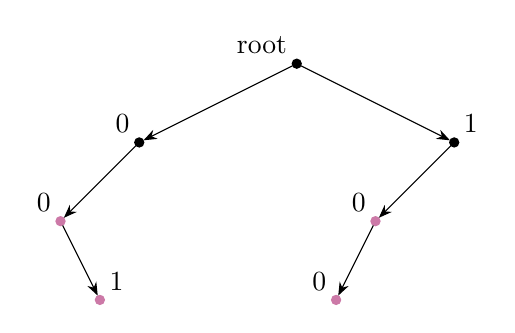
\begin{tikzpicture}
  \node[dot] (p) at (0, 0)       {};
  \node[dot] (l) at (-2, -1)     {}  edge[<-] (p);
  \node[dot,cbReddischPurple] (ll) at (-3, -2)  {}  edge[<-] (l);
  \node[dot,cbReddischPurple] (llr) at (-2.5, -3) {}  edge[<-] (ll);
  \node[dot] (r) at (2, -1)     {}  edge[<-] (p);
  \node[dot,cbReddischPurple] (rl) at (1, -2)  {}  edge[<-] (r);
  \node[dot,cbReddischPurple] (rll) at (0.5, -3) {} edge[<-] (rl);


  \node[above left] at (p)  {root};
  \node[above left] at (l)  {0};
  \node[above left] at (ll) {0};
  \node[above right] at (llr) {1};
  \node[above right] at (r)  {1};
  \node[above left] at (rl) {0};
  \node[above left] at (rll) {0};
\end{tikzpicture}

Adding:

To add a bitstring, you must traverse the path in relation to the new bitstring, and for any bit that isn't already in the data structure, add it. Once reaching the terminal bit of the bitstring, make the last node a red node.
This traverses the tree only for the amount of bits in the bitstring, making it $\sim N$ complexity.

ex. Adding bitstring "1100", traverse tree 1->1->0->0, and for any non-existance node, create it. Make the last 0 a red node.

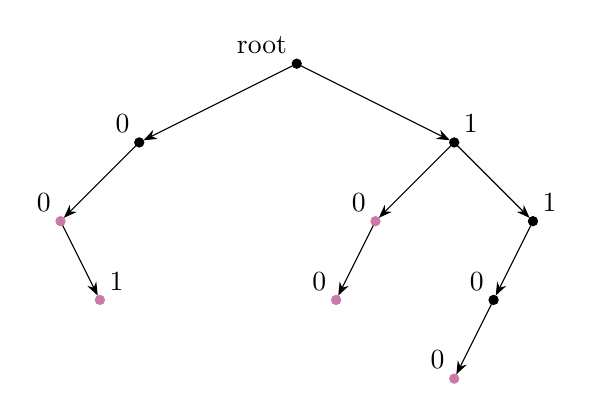
\begin{tikzpicture}
  \node[dot] (p) at (0, 0)       {};
  \node[dot] (l) at (-2, -1)     {}  edge[<-] (p);
  \node[dot,cbReddischPurple] (ll) at (-3, -2)  {}  edge[<-] (l);
  \node[dot,cbReddischPurple] (llr) at (-2.5, -3) {}  edge[<-] (ll);
  \node[dot] (r) at (2, -1)     {}  edge[<-] (p);
  \node[dot,cbReddischPurple] (rl) at (1, -2)  {}  edge[<-] (r);
  \node[dot,cbReddischPurple] (rll) at (0.5, -3) {} edge[<-] (rl);
  \node[dot] (rr) at (3, -2) {} edge[<-] (r);
  \node[dot] (rrl) at (2.5, -3) {} edge[<-] (rr);
  \node[dot,cbReddischPurple] (rrll) at (2, -4) {} edge[<-] (rrl);


  \node[above left] at (p)  {root};
  \node[above left] at (l)  {0};
  \node[above left] at (ll) {0};
  \node[above right] at (llr) {1};
  \node[above right] at (r)  {1};
  \node[above left] at (rl) {0};
  \node[above left] at (rll) {0};
  \node[above right] at (rr) {1};
  \node[above left] at (rrl) {0};
  \node[above left] at (rrll) {0};
\end{tikzpicture}

Removing:

To remove a bitstring, you traverse the path representing the bitstring to remove. Once reaching the last node, remove that node only if it has no children, else turn it from a red to black node. This takes $\OOG{N}$ as you are traversing the tree downwards via length of the binary string. Then recursively retraverse the tree upwards and for every node that has no children, delete that node from the tree. This is also $\OOG{N}$ complexity as you are traversing the same path as before, which makes the entire thing $\OOG{2N}$ which equals $\OOG{N}$.

The previous method was the more neat way to keep the tree clean, however, it suffices to just traverse the tree and turn the terminal bit from a red node to a black one. In either case, you go down/up the tree max twice, making it $\sim N$ complexity.

Contains:

Traverse the tree representing the bitstring to check. If there is any element in the bitstring that does not exist in the path, return false. If all bitstrings are in the tree, once you reach the last node, check if the node is red. If it is red, return true, else return false.

This is a $\sim N$ complexity as you only need to traverse one path of the tree as long as the bitstring you are checking. 

\item Let $W$ of length $\abs{W} = N$ be a binary string and let $S$ be a \AName{BSSet} set. Provide an algorithm that prints all strings $V \in S$ that start with the prefix $W$ (the first $\abs{W}$ characters of $S$ are equivalent to $W$). Your algorithm should have a worst-case complexity of $\OOG{N + k}$ in which $k$ is the number of characters printed to the output.

Assumption: The prefix exists in the tree. If needed, this can be checked before the algorithm in $\sim N$ as showed in q4.1, so the complexity won't change. This is done in the following algo.

\begin{myalgo}{\AName{PrintPrefix}($\VAR{node},\VAR{string}$)}
  \IF{$\VAR{node}=\Null$ \OR $!contains(\VAR{string})$}
    \RETURN
  \ENDIF

  \IF{$\VAR{node}=\VAR{root}$}
    \STATE $\VAR{currNode} = root$
    \STATE $\VAR{prefix} = \VAR{string}$
    \STATE $\VAR{string} = ""$

    \COMMENT{//loop through prefix and traverse the tree while appending each value to string.}
    \FOR{$char \in \VAR{prefix}$}
      \IF{$\VAR{char}="0"$}
        \STATE $\VAR{currNode} = \VAR{currNode.left}$
      \ELSIF{$\VAR{char}="1"$}
        \STATE $\VAR{currNode} = \VAR{currNode.right}$
      \ENDIF
      \STATE $\VAR{string}.append(currNode.data)$
    \ENDFOR

    \IF{$currNode.color == "red"$}
      \PRINT $string$ \COMMENT{//this is to handle printing the prefix if it is in the tree.}
    \ENDIF

    \STATE \AName{PrintPrefix($currNode.left, currNode.data+""$)} \COMMENT{//print all bitstrings in left subtree}
    \STATE \AName{PrintPrefix($currNode.right, currNode.data+""$)} \COMMENT{//print all bitstrings in right subtree}
  \ELSE
    \STATE $\VAR{string}.append(node.data)$ \COMMENT{//Add current node data to string}
    \IF{$node.color = "red"$}
      \STATE \COMMENT{//if current node is a terminal node, print its string (the path traversed to get here)}
      \PRINT $string$
    \ENDIF

    \STATE \AName{PrintPrefix($currNode.left, currNode.data+""$)} \COMMENT{//print all bitstrings in left subtree}
    \STATE \AName{PrintPrefix($currNode.right, currNode.data+""$)} \COMMENT{//print all bitstrings in right subtree}
  \ENDIF
\end{myalgo}

You can call the method via \AName{PrintPrefix}($\VAR{root}, prefix$). The complexity is $\sim N + k$ since the algorithm traverses the path of the given prefix which is $\sim N$. Then it traverses every path below it recursively. Anytime it gets to a red node, it prints out the path it took to get there, including the current node (note: it does not need to retraverse the graph backwards as it holds the path in a string). This second part is $\OOG{k}$ as it checks only all characters after the prefix. 
As long as the data structure makes sure to only have paths that have a red node at the end (explained in q4.1 where deleting a string will remove all terminal black nodes), it will always be $\sim k$ since the longest path to traverse is as long as the largest binary string to print. 

\item Professor X claims to have developed a data structure \AName{BSSetX} to which any binary string $W$ of length $\abs{W} = N$ can be added in $\OOG{N}$. Furthermore, Professor X claims that \AName{BSSetX}  provides \emph{ordered iteration}: one can iterate over all $M = \abs{S}$ strings in a set $S$, implemented via \AName{BSSetX}, in a lexicographical order in $\OOG{M + T}$ in which $T$ is the combined length of the $M$ strings. Professor X claims that this method of sorting binary strings proves that the worst-case lower bound for sorting $M$ binary strings is \emph{not} $\OOG{M \log_2(M)}$ comparisons. Argue why Professor X is wrong.

We note that strings $S_1$ and $S_2$ are \emph{lexicographical ordered}, denoted by $S_1 \prec S_2$, if $S_1$ comes before $S_2$ in an alphabetical sort (e.g., as used in a dictionary). Next, we formalize $S_1 \prec S_2$ for binary strings: we have $S_1 \prec S_2$ if $S_1$ and $S_2$ are equivalent up to the $0\leq i \leq \min(\abs{S_1}, \abs{S_2})$-th character ($S_1[0] = S_2[0]$,
\dots, $S_1[i-1] = S_2[i-1]$) and either $\abs{S_1} = i < \abs{S_2}$ or the $(i+1)$-th character of $S_1$ comes before the $(i+1)$-th character of $S_2$ (in which case $S_1[i] = 0$ and $S_2[i] = 1$). For example, $0 \prec 00$ and $00 \prec 01$, but not $100 \prec 10$. 

a) Given a binary string of length $N$, adding takes $\OOG{N}$ time.
Now given there is a list of $M$ binary strings all of length $N$, the complexity for adding all the binary strings to the data structure would be $\OOG{M} \cdot N$, where $N,M \in \mathbb{N}$. Let's say $N = M$, in that case, we can already see our complexity would be $\OOG{M^2}$ just to add the strings to the data structure, where $\OOG{M^2} \geq \OOG{M \log_2(M)}$.
Furthermore, $T$ is the combined length of all binary strings to add, which would again be $M \cdot N$. Again we can see $\exists N, N>M \log_2(M)$ (ex. $N = M$), then this will be greater than the bound set by the Professor.
Also the complexity of this algorithm relies on $T$ which is the combined length of the strings. Professor X assumes that $T < log_2{M}$, $\forall T,M \in \mathbb{N}$, which is not always the case, especially if you have larger binary strings. \\

b) Now to tackle this for all inputs:

We need to prove that $\sim M + MN \geq M log_2{M}$ for all cases, where $M$ is the number of binary strings in the input and $N$ is the length of a string. We will look into general cases where the length of all binary strings are the same. It doesn't change anything, since if you take the same argument for the smallest binary sting in the input, it would be the same.

Since we are dealing with binary strings, we know the maximum M for any N is $2^N$ since there are 2 choices per each bit. We will say the minimum $M$ is 2 to make $log_2{M}$ easier.

For the minimum $M=2$:\\
$M + MN \geq M log_2{M}$\\
$2 + 2N \geq 2 log_2{2}$\\
$2 + 2N \geq 2$

Which is always true for any positive $N$.

For the maximum $M=2^N$:\\
$M + MN \geq M log_2{M}$\\
$2^N + 2^{N}N \geq 2^N log_2{2^N}$\\
$\sim 2^{N}N \geq 2^{N} Nlog_2{2}$\\
$\sim 2^{N}N \geq 2^{N} N$\\

Which is also always true.

To conclude, we have just proven for all lengths of binary strings, Professor X simply cannot beat $M log_2{M}$.

\end{questions}
\end{problem}

\SUBMITMSG{}
\DEFAULTGRADING{}

\end{document}